% questions.tex —— 2017 年·全国Ⅱ卷·文科 · 题目内容片段（无答案）
% 由 tools/generate_projects.py 依来源总账自 2017/2017_数学真题_全国2文_试题.md 生成，勿手改（改源 MD 后重跑）


\gkpart{数学}

\begin{gktip}
\textbf{来源说明}：本题面依据固定源 PDF 两页 A3 页面逐题核对，原卷印刷页码 1043–1044。固定源不附答案；本文件仅为题面规范源。
\end{gktip}

\gkpart{一、选择题}

\begin{question}
\gkti{1}设集合 \(A=\{1,2,3\}\)，\(B=\{2,3,4\}\)，则 \(A\cup B=\)（　）

（A）\(\{1,2,3,4\}\)　（B）\(\{1,2,3\}\)　（C）\(\{2,3,4\}\)　（D）\(\{1,3,4\}\)

\end{question}
\begin{question}
\gkti{2}\((1+i)(2+i)=\)（　）

（A）\(1-i\)　（B）\(1+3i\)　（C）\(3+i\)　（D）\(3+3i\)

\end{question}
\begin{question}
\gkti{3}函数 \(f(x)=\sin\left(2x+\dfrac{\pi}{3}\right)\) 的最小正周期为（　）

（A）\(4\pi\)　（B）\(2\pi\)　（C）\(\pi\)　（D）\(\dfrac{\pi}{2}\)

\end{question}
\begin{question}
\gkti{4}设非零向量 \(\boldsymbol a,\boldsymbol b\) 满足 \(|\boldsymbol a+\boldsymbol b|=|\boldsymbol a-\boldsymbol b|\)，则（　）

（A）\(\boldsymbol a\perp\boldsymbol b\)　（B）\(|\boldsymbol a|=|\boldsymbol b|\)　（C）\(\boldsymbol a\parallel\boldsymbol b\)　（D）\(|\boldsymbol a|>|\boldsymbol b|\)

\end{question}
\begin{question}
\gkti{5}若 \(a>1\)，则双曲线 \(\dfrac{x^2}{a^2}-y^2=1\) 的离心率的取值范围是（　）

（A）\((\sqrt2,+\infty)\)　（B）\((\sqrt2,2)\)　（C）\((1,\sqrt2)\)　（D）\((1,2)\)

\Needspace{0.4\textheight}
\end{question}
\begin{question}
\gkti{6}如图，网格纸上小正方形的边长为 \(1\)，粗实线画出的是某几何体的三视图，该几何体由一平面将一圆柱截去一部分后所得，则该几何体的体积为（　）
\nopagebreak[4]
\begin{center}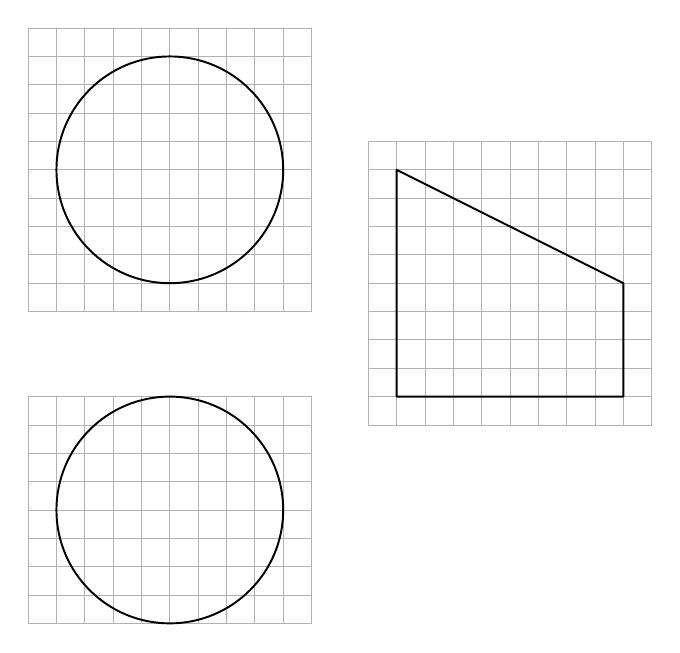
\begin{tikzpicture}[line cap=round,line join=round,line width=0.7pt,scale=0.36]
\begin{scope}[shift={(0,11)}]
  \draw[gray!60,line width=0.3pt] (0,0) grid (10,10);
  \draw (5,5) circle (4);
\end{scope}
\begin{scope}[shift={(12,7)}]
  \draw[gray!60,line width=0.3pt] (0,0) grid (10,10);
  \draw (1,1)--(9,1)--(9,5)--(1,9)--cycle;
\end{scope}
\begin{scope}
  \draw[gray!60,line width=0.3pt] (0,0) grid (10,8);
  \draw (5,4) circle (4);
\end{scope}
\end{tikzpicture}
\end{center}
\nopagebreak[4]
（A）\(90\pi\)　（B）\(63\pi\)　（C）\(42\pi\)　（D）\(36\pi\)

\end{question}
\begin{question}
\gkti{7}设 \(x,y\) 满足约束条件
\nopagebreak[4]
\[
\begin{cases}
2x+3y-3\le 0,\\
2x-3y+3\ge 0,\\
y+3\ge 0,
\end{cases}
\]
则 \(z=2x+y\) 的最小值是（　）

（A）\(-15\)　（B）\(-9\)　（C）\(1\)　（D）\(9\)

\end{question}
\begin{question}
\gkti{8}函数 \(f(x)=\ln(x^2-2x-8)\) 的单调递增区间为（　）

（A）\((-\infty,-2)\)　（B）\((-\infty,1)\)　（C）\((1,+\infty)\)　（D）\((4,+\infty)\)

\end{question}
\begin{question}
\gkti{9}甲、乙、丙、丁四位同学一起去向老师询问成语竞赛的成绩。老师说：你们四人中有2位优秀，2位良好，我现在给甲看乙、丙的成绩，给乙看丙的成绩，给丁看甲的成绩。看后甲对大家说：我还是不知道我的成绩。根据以上信息，则（　）

（A）乙可以知道四人的成绩　（B）丁可以知道四人的成绩　（C）乙、丁可以知道对方的成绩　（D）乙、丁可以知道自己的成绩

\Needspace{0.4\textheight}
\end{question}
\begin{question}
\gkti{10}执行如图的程序框图，如果输入的 \(a=-1\)，则输出的 \(S=\)（　）
\nopagebreak[4]
\begin{center}\begin{tikzpicture}[line width=0.75pt,line cap=round,line join=round,font=\small]
\node[draw,rounded corners,minimum width=1.35cm,minimum height=0.5cm] (start) at (0,0) {开始};
\node[draw,minimum width=2.2cm,minimum height=0.55cm] (input) at (0,-0.95) {输入 $a$};
\node[draw,minimum width=2.7cm,minimum height=0.55cm] (init) at (0,-1.9) {$S=0,\ K=1$};
\coordinate (dt) at (0,-2.6);
\coordinate (dr) at (1.9,-3.2);
\coordinate (db) at (0,-3.8);
\coordinate (dl) at (-1.9,-3.2);
\draw (dt)--(dr)--(db)--(dl)--cycle;
\node at (0,-3.2) {$K\le 6$};
\node[draw,minimum width=3.0cm,minimum height=0.55cm] (sum) at (0,-4.55) {$S=S+a\cdot K$};
\node[draw,minimum width=2.3cm,minimum height=0.55cm] (flip) at (0,-5.45) {$a=-a$};
\node[draw,minimum width=2.6cm,minimum height=0.55cm] (next) at (0,-6.35) {$K=K+1$};
\node[draw,minimum width=1.9cm,minimum height=0.55cm] (out) at (3.6,-3.2) {输出 $S$};
\node[draw,rounded corners,minimum width=1.35cm,minimum height=0.5cm] (end) at (3.6,-4.2) {结束};
\draw[->] (start)--(input);
\draw[->] (input)--(init);
\draw[->] (init)--(dt);
\draw[->] (db)--node[right]{是}(sum);
\draw[->] (sum)--(flip);
\draw[->] (flip)--(next);
\draw[->] (next.west)--(-2.65,-6.35)--(-2.65,-3.2)--(dl);
\draw[->] (dr)--node[above]{否}(out.west);
\draw[->] (out)--(end);
\end{tikzpicture}
\end{center}
\nopagebreak[4]
（A）\(2\)　（B）\(3\)　（C）\(4\)　（D）\(5\)

\end{question}
\begin{question}
\gkti{11}从分别写有1，2，3，4，5的5张卡片中随机抽取1张，放回后再随机抽取1张，则抽得的第一张卡片上的数大于第二张卡片上的数的概率为（　）

（A）\(\dfrac{1}{10}\)　（B）\(\dfrac{1}{5}\)　（C）\(\dfrac{3}{10}\)　（D）\(\dfrac{2}{5}\)

\end{question}
\begin{question}
\gkti{12}过抛物线 \(C:y^2=4x\) 的焦点 \(F\)，且斜率为 \(\sqrt3\) 的直线交 \(C\) 于点 \(M\)（\(M\) 在 \(x\) 轴上方），\(l\) 为 \(C\) 的准线，点 \(N\) 在 \(l\) 上，且 \(MN\perp l\)，则 \(M\) 到直线 \(NF\) 的距离为（　）

（A）\(\sqrt5\)　（B）\(2\sqrt2\)　（C）\(2\sqrt3\)　（D）\(3\sqrt3\)

\end{question}
\gkpart{二、填空题}

\begin{question}
\gkti{13}函数 \(f(x)=2\cos x+\sin x\) 的最大值为\gkblank{}。

\end{question}
\begin{question}
\gkti{14}已知函数 \(f(x)\) 是定义在 \(\mathbb R\) 上的奇函数，当 \(x\in(-\infty,0)\) 时，\(f(x)=2x^3+x^2\)，则 \(f(2)=\)\gkblank{}。

\end{question}
\begin{question}
\gkti{15}长方体的长、宽、高分别为3，2，1，其顶点都在球 \(O\) 的球面上，则球 \(O\) 的表面积为\gkblank{}。

\end{question}
\begin{question}
\gkti{16}\(\triangle ABC\) 的内角 \(A,B,C\) 的对边分别为 \(a,b,c\)，若 \(2b\cos B=a\cos C+c\cos A\)，则 \(B=\)\gkblank{}。

\end{question}
\gkpart{三、解答题}

\begin{question}
\gkti{17}已知等差数列 \(\{a_n\}\) 的前 \(n\) 项和为 \(S_n\)，等比数列 \(\{b_n\}\) 的前 \(n\) 项和为 \(T_n\)，\(a_1=-1,b_1=1,a_2+b_2=2\)。

（1） 若 \(a_3+b_3=5\)，求 \(\{b_n\}\) 的通项公式；

（2） 若 \(T_3=21\)，求 \(S_3\)。

\Needspace{0.4\textheight}
\end{question}
\begin{question}
\gkti{18}如图，四棱锥 \(P-ABCD\) 中，侧面 \(PAD\) 为等边三角形且垂直于底面 \(ABCD\)，\(AB=BC=\dfrac12 AD\)，\(\angle BAD=\angle ABC=90^\circ\)。
\nopagebreak[4]
\begin{center}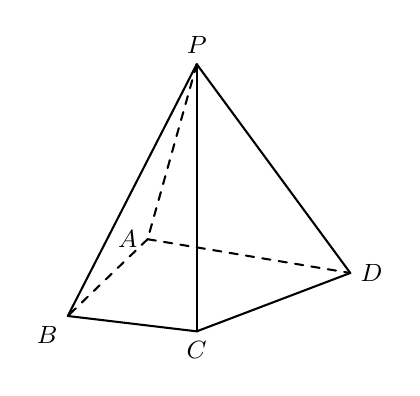
\begin{tikzpicture}[x=0.78cm,y=0.78cm,line cap=round,line join=round,line width=0.75pt,font=\small]
\coordinate (A) at (1.3,1.25);
\coordinate (B) at (0,0);
\coordinate (C) at (2.1,-0.25);
\coordinate (D) at (4.6,0.7);
\coordinate (P) at (2.1,4.1);
\draw (P)--(B)--(C)--(D)--(P);
\draw (P)--(C);
\draw[dashed] (P)--(A);
\draw[dashed] (A)--(B);
\draw[dashed] (A)--(D);
\node[above] at (P) {$P$};
\node[below left] at (B) {$B$};
\node[below] at (C) {$C$};
\node[right] at (D) {$D$};
\node[left] at (A) {$A$};
\end{tikzpicture}
\end{center}
\nopagebreak[4]
（1） 证明：直线 \(BC\parallel\) 平面 \(PAD\)；

（2） 若 \(\triangle PCD\) 面积为 \(2\sqrt7\)，求四棱锥 \(P-ABCD\) 的体积。

\Needspace{0.4\textheight}
\end{question}
\begin{question}
\gkti{19}海水养殖场进行某水产品的新、旧网箱养殖方法的产量对比，收获时各随机抽取了100个网箱，测量各箱水产品的产量（单位：kg），其频率分布直方图如图。
\nopagebreak[4]
\begin{center}\begin{tikzpicture}[x=0.68cm,y=0.68cm,line width=0.55pt,font=\scriptsize]
\begin{scope}
  \draw[->] (0,0)--(9.45,0);
  \draw[->] (0,0)--(0,7.55);
  \foreach \y/\lab/\x in {1.2/0.012/0,1.4/0.014/-1,2.0/0.020/0,2.4/0.024/0,3.2/0.032/0,3.4/0.034/-1,4.0/0.040/0} {
    \draw[densely dashed,gray] (0,\y)--(9,\y);
    \node[left] at (\x,\y) {\lab};
  }
  \foreach \x/\lab in {0/25,1/30,2/35,3/40,4/45,5/50,6/55,7/60,8/65,9/70} {
    \draw (\x,0)--(\x,-0.08);
    \node[below] at (\x,-0.12) {\lab};
  }
  \foreach \x/\h in {0/1.2,1/1.4,2/2.4,3/3.4,4/4.0,5/3.2,6/2.0,7/1.2,8/1.2} {
    \draw[fill=white] (\x,0) rectangle ++(1,\h);
  }
  \node[anchor=west] at (0.18,7.15) {频率/组距};
  \node at (4.5,-0.9) {箱产量/kg};
  \node at (4.5,-1.55) {旧养殖法};
\end{scope}
\begin{scope}[shift={(12,0)}]
  \draw[->] (0,0)--(7.45,0);
  \draw[->] (0,0)--(0,7.55);
  \foreach \y/\lab/\x in {0.4/0.004/0,0.8/0.008/-1,1.0/0.010/0,2.0/0.020/0,4.4/0.044/0,4.6/0.046/-1,6.8/0.068/0} {
    \draw[densely dashed,gray] (0,\y)--(7,\y);
    \node[left] at (\x,\y) {\lab};
  }
  \foreach \x/\lab in {0/35,1/40,2/45,3/50,4/55,5/60,6/65,7/70} {
    \draw (\x,0)--(\x,-0.08);
    \node[below] at (\x,-0.12) {\lab};
  }
  \foreach \x/\h in {0/0.4,1/2.0,2/4.4,3/6.8,4/4.6,5/1.0,6/0.8} {
    \draw[fill=white] (\x,0) rectangle ++(1,\h);
  }
  \node[anchor=west] at (0.18,7.15) {频率/组距};
  \node at (3.5,-0.9) {箱产量/kg};
  \node at (3.5,-1.55) {新养殖法};
\end{scope}
\end{tikzpicture}
\end{center}
\nopagebreak[4]
（1） 记 \(A\) 表示事件“旧养殖法的箱产量低于50 kg”，估计 \(A\) 的概率；

（2） 填写下面列联表，并根据列联表判断是否有99\%的把握认为箱产量与养殖方法有关；

\begin{center}
\begin{tabular}{lrr}
\toprule
 & 箱产量 < 50 kg & 箱产量 $\geq$ 50 kg \\
\midrule
旧养殖法 &  &  \\
新养殖法 &  &  \\
\bottomrule
\end{tabular}
\end{center}

（3） 根据箱产量的频率分布直方图，求新养殖法箱产量的优劣进行比较。

\Needspace{10\baselineskip}
附：

\begin{center}
\begin{tabular}{lrrr}
\toprule
\(P(K^2\ge k)\) & 0.050 & 0.010 & 0.001 \\
\midrule
\(K\) & 3.841 & 6.635 & 10.828 \\
\bottomrule
\end{tabular}
\end{center}

\nopagebreak[4]
\[
K^2=\frac{n(ad-bc)^2}{(a+b)(c+d)(a+c)(b+d)}.
\]

\end{question}
\begin{question}
\gkti{20}设 \(O\) 为坐标原点，动点 \(M\) 在椭圆 \(C:\dfrac{x^2}{2}+y^2=1\) 上，过 \(M\) 作 \(x\) 轴的垂线，垂足为 \(N\)，点 \(P\) 满足 \(\overrightarrow{NP}=\sqrt2\,\overrightarrow{NM}\)。

（1） 求点 \(P\) 的轨迹方程；

（2） 设点 \(Q\) 在直线 \(x=-3\) 上，且 \(\overrightarrow{OP}\cdot\overrightarrow{PQ}=1\)。证明：过点 \(P\) 且垂直于 \(OQ\) 的直线 \(l\) 过 \(C\) 的左焦点 \(F\)。

\end{question}
\begin{question}
\gkti{21}设函数 \(f(x)=(1-x^2)e^x\)。

（1） 讨论 \(f(x)\) 的单调性；

（2） 当 \(x\ge0\) 时，\(f(x)\le ax+1\)，求 \(a\) 的取值范围。

\end{question}
\begin{question}
\gkti{22}在直角坐标系 \(xOy\) 中，以坐标原点为极点，\(x\) 轴的正半轴为极轴建立极坐标系，曲线 \(C_1\) 的极坐标方程为 \(\rho\cos\theta=4\)。

（1） \(M\) 为曲线 \(C_1\) 上的动点，点 \(P\) 在线段 \(OM\) 上，且满足 \(|OM|\cdot|OP|=16\)，求点 \(P\) 的轨迹 \(C_2\) 的直角坐标方程；

（2） 设点 \(A\) 的极坐标为 \(\left(2,\dfrac{\pi}{3}\right)\)，点 \(B\) 在曲线 \(C_2\) 上，求 \(\triangle OAB\) 面积的最大值。

\end{question}
\begin{question}
\gkti{23}已知 \(a>0,b>0,a^3+b^3=2\)，证明：

（1） \((a+b)(a^5+b^5)\ge4\)；

（2） \(a+b\le2\)。

\end{question}